% pySeqAlign -- overview presentation (Beamer + TikZ)
% Build: latexmk -pdf pyseqalign_overview.tex   (or pdflatex x2)
\documentclass[aspectratio=169,10pt]{beamer}

\usepackage[T1]{fontenc}
\usepackage{lmodern}
\usepackage{booktabs}
\usepackage{graphicx}
\usepackage{tikz}
\usetikzlibrary{positioning,arrows.meta,fit,backgrounds,calc,shapes.geometric,shadows.blur}
\usepackage{listings}
\lstdefinestyle{py}{language=Python,basicstyle=\ttfamily\small,
  keywordstyle=\color{psaBlue}\bfseries,stringstyle=\color{psaRed},
  commentstyle=\color{psaGray}\itshape,showstringspaces=false,
  columns=fullflexible,keepspaces=true}

\usetheme{Madrid}
\definecolor{psaBlue}{HTML}{1F4E79}
\definecolor{psaAcc}{HTML}{1F77B4}
\definecolor{psaGreen}{HTML}{2CA02C}
\definecolor{psaRed}{HTML}{C0392B}
\definecolor{psaGray}{HTML}{555555}
\setbeamercolor{structure}{fg=psaBlue}
\setbeamercolor{frametitle}{bg=psaBlue,fg=white}
\setbeamertemplate{navigation symbols}{}
\setbeamertemplate{itemize items}[circle]
\setbeamerfont{frametitle}{size=\large,series=\bfseries}

\newcommand{\code}[1]{\texttt{\small #1}}
\newcommand{\atom}[1]{\texttt{#1}}

\title[pySeqAlign]{\textbf{pySeqAlign}}
\subtitle{Relational sequence alignment, multiple alignment, and logos}
\author{A.\ Karwath}
\institute{\small github.com/athro/pySeqAlign \quad$\cdot$\quad PyPI: \texttt{pyseqalignment}}
\date{}

\begin{document}

{\setbeamertemplate{footline}{}
\begin{frame}[plain]
  \titlepage
  \begin{center}\small
  \emph{Aligning sequences of structured logical atoms} --- the ILP-2006 layer:\\
  Karwath \& Kersting, \textit{Relational Sequence Alignments and Logos} (ILP 2006).
  \end{center}
\end{frame}}

\begin{frame}{Outline}
  \tableofcontents
\end{frame}

% ============================================================
\section{What pySeqAlign does}
\begin{frame}{What pySeqAlign does}
  A \alert{domain-independent} sequence-alignment library that works on
  \textbf{structured} elements (logical atoms), not just flat symbols.
  \vspace{0.4em}
  \begin{columns}[T]
    \begin{column}{0.54\textwidth}
      \begin{itemize}
        \item \textbf{Alignment}: Needleman--Wunsch (linear \& affine gaps),
              Smith--Waterman (k-best local).
        \item \textbf{Relational distance}: Nienhuys--Cheng distance over
              logical atoms $\Rightarrow$ similarity $S=1-d$.
        \item \textbf{Substitution matrices}: BLOSUM / PAM bundled.
        \item \textbf{Multiple alignment}: progressive MSA over a
              neighbour-joining guide tree.
        \item \textbf{Relational logos}: information-content logos of aligned
              atoms (+ per-column least-general generalisation).
        \item \textbf{ILP backends}: Aleph / Popper (optional, SWI-Prolog).
        \item \textbf{Optional C++ aligner}: pybind11 affine kernel,
              $\sim$100--270$\times$ faster, auto-compiled on install.
      \end{itemize}
    \end{column}
    \begin{column}{0.46\textwidth}
      \centering
      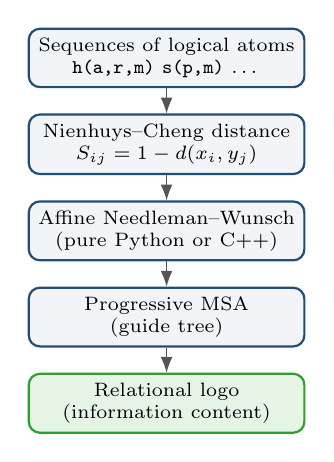
\begin{tikzpicture}[font=\scriptsize,node distance=3.2mm,
        box/.style={draw=psaBlue,thick,rounded corners,fill=psaBlue!6,
                    minimum width=3.5cm,minimum height=0.72cm,align=center}]
        \node[box] (a) {Sequences of logical atoms\\\atom{h(a,r,m)} \atom{s(p,m)} \dots};
        \node[box,below=of a] (d) {Nienhuys--Cheng distance\\$S_{ij}=1-d(x_i,y_j)$};
        \node[box,below=of d] (al) {Affine Needleman--Wunsch\\(pure Python or C++)};
        \node[box,below=of al] (m) {Progressive MSA\\(guide tree)};
        \node[box,below=of m,fill=psaGreen!12,draw=psaGreen] (lo) {Relational logo\\(information content)};
        \draw[-{Latex[length=2mm]},psaGray] (a)--(d);
        \draw[-{Latex[length=2mm]},psaGray] (d)--(al);
        \draw[-{Latex[length=2mm]},psaGray] (al)--(m);
        \draw[-{Latex[length=2mm]},psaGray] (m)--(lo);
      \end{tikzpicture}
    \end{column}
  \end{columns}
\end{frame}

% ============================================================
\section{Sequence alignment}
\begin{frame}{Global alignment: Needleman--Wunsch}
  Fill a DP matrix; each cell takes the best of three moves
  (match/mismatch, gap in one sequence, gap in the other):
  \vspace{0.5em}
  \begin{columns}[c]
    \begin{column}{0.52\textwidth}
      \centering
      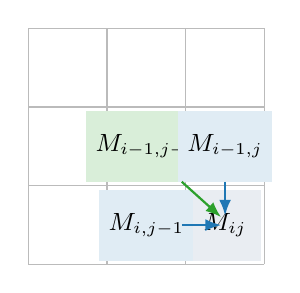
\begin{tikzpicture}[font=\small]
        \foreach \i in {0,1,2,3} \draw[psaGray!40] (\i,0)--(\i,3);
        \foreach \j in {0,1,2,3} \draw[psaGray!40] (0,\j)--(3,\j);
        \node[fill=psaBlue!10,minimum size=0.9cm] at (2.5,0.5) {$M_{ij}$};
        \node[fill=psaGreen!18,minimum size=0.9cm] at (1.5,1.5) {$M_{i\text{-}1,j\text{-}1}$};
        \node[fill=psaAcc!14,minimum size=0.9cm] at (1.5,0.5) {$M_{i,j\text{-}1}$};
        \node[fill=psaAcc!14,minimum size=0.9cm] at (2.5,1.5) {$M_{i\text{-}1,j}$};
        \draw[-{Latex[length=2mm]},psaGreen,thick] (1.95,1.05)--(2.45,0.6);
        \draw[-{Latex[length=2mm]},psaAcc,thick] (1.95,0.5)--(2.45,0.5);
        \draw[-{Latex[length=2mm]},psaAcc,thick] (2.5,1.05)--(2.5,0.62);
      \end{tikzpicture}
    \end{column}
    \begin{column}{0.46\textwidth}
      \[
        M_{ij}=\max\!\begin{cases}
          M_{i\text{-}1,j\text{-}1}+S_{ij} & \text{(diag: match)}\\[2pt]
          M_{i,j\text{-}1}+w & \text{(gap in seq.\ 1)}\\[2pt]
          M_{i\text{-}1,j}+w & \text{(gap in seq.\ 2)}
        \end{cases}
      \]
      \vspace{0.4em}
      \small
      \begin{itemize}
        \item \textbf{Affine gaps}: separate open/extend costs (3-matrix
              $M/I_x/I_y$ recurrence) -- \code{NeedlemanWunschAffine}.
        \item \textbf{Local}: Smith--Waterman with k-best non-overlapping hits.
        \item The score $S_{ij}$ is \emph{pluggable} -- this is the hook for
              relational distances.
      \end{itemize}
    \end{column}
  \end{columns}
\end{frame}

% ============================================================
\section{Relational distance}
\begin{frame}{From flat symbols to logical atoms}
  Real sequences carry internal structure. An SSE or a tagged word is an
  \alert{atom}, not a letter:
  \begin{center}\small
    \atom{he(h(right,alpha),long)}\qquad \atom{st(parallel,short)}\qquad
    \atom{nn(balloon)}\qquad \atom{vbd(blew)}
  \end{center}
  \vspace{0.3em}
  The \textbf{Nienhuys--Cheng} distance treats a ground atom as a hierarchy:
  same functor $\Rightarrow$ distance shrinks with the fraction of matching
  arguments (at most $0.5$); different functor $\Rightarrow$ distance $1$.
  \[
    d(p(t_1,\dots,t_n),p(s_1,\dots,s_n))=\tfrac{1}{2n}\sum_{i=1}^{n} d(t_i,s_i),
    \qquad d(p,q)=1\ \text{if } p\neq q .
  \]
  \begin{columns}[c]
    \begin{column}{0.5\textwidth}
      \centering
      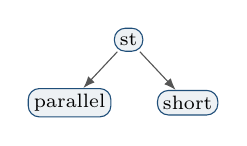
\begin{tikzpicture}[font=\scriptsize,level distance=8mm,
        every node/.style={draw=psaBlue,rounded corners,fill=psaBlue!8,inner sep=2pt},
        edge from parent/.style={draw=psaGray,-{Latex[length=1.5mm]}}]
        \node {st}
          child {node {parallel}}
          child {node {short}};
      \end{tikzpicture}\\[-0.2em]
      {\scriptsize \atom{st(parallel,short)}}
    \end{column}
    \begin{column}{0.5\textwidth}
      \small
      Used as alignment score: $S_{ij}=1-d(x_i,y_j)$.
      \\[0.3em]
      \emph{Example:} $d(\atom{st(parallel,short)},\atom{st(parallel,long)})
        =\tfrac{1}{4}(0+1)=0.25 \Rightarrow S=0.75$.
      \\[0.3em]
      Implemented in \code{pyseqalign.scoring.distance.AtomDistance}.
    \end{column}
  \end{columns}
\end{frame}

% ============================================================
\section{Multiple alignment}
\begin{frame}{Multiple sequence alignment}
  Progressive MSA: all-pairs distances $\rightarrow$ neighbour-joining guide
  tree $\rightarrow$ merge along the tree. Parameterised by \alert{any} scoring
  function.
  \begin{center}
    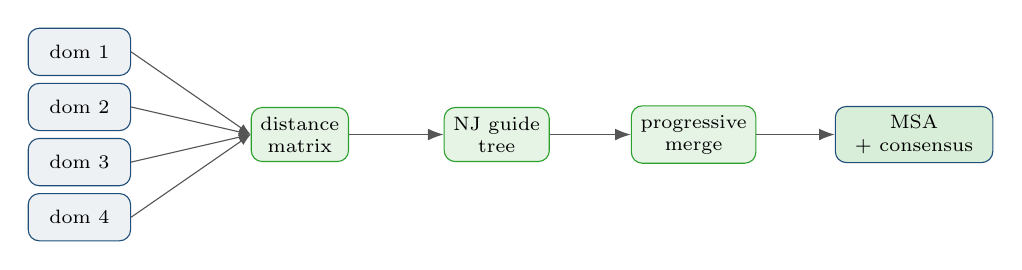
\begin{tikzpicture}[font=\scriptsize,
      seq/.style={draw=psaBlue,fill=psaBlue!8,rounded corners,align=center,minimum height=0.6cm,minimum width=1.3cm},
      op/.style={draw=psaGreen,fill=psaGreen!12,rounded corners,align=center,minimum height=0.6cm}]
      \node[seq] (s1) at (0,2.1) {dom 1};
      \node[seq] (s2) at (0,1.4) {dom 2};
      \node[seq] (s3) at (0,0.7) {dom 3};
      \node[seq] (s4) at (0,0.0) {dom 4};
      \node[op] (dm) at (2.8,1.05) {distance\\matrix};
      \node[op] (gt) at (5.3,1.05) {NJ guide\\tree};
      \node[op] (pm) at (7.8,1.05) {progressive\\merge};
      \node[seq,fill=psaGreen!18,minimum width=2.0cm] (out) at (10.6,1.05) {MSA\\+ consensus};
      \foreach \s in {s1,s2,s3,s4} \draw[-{Latex[length=1.5mm]},psaGray] (\s.east)--(dm.west);
      \draw[-{Latex[length=2mm]},psaGray] (dm)--(gt);
      \draw[-{Latex[length=2mm]},psaGray] (gt)--(pm);
      \draw[-{Latex[length=2mm]},psaGray] (pm)--(out);
    \end{tikzpicture}
  \end{center}
  \vspace{-0.2em}
  \begin{block}{Why ``any scoring function'' matters}
    The same MSA accepts the fixed Nienhuys--Cheng distance \emph{or} a reward
    matrix \alert{learned by pyREAL's boosting} -- one MSA engine, two regimes.
  \end{block}
\end{frame}

% ============================================================
\section{Relational logos}
\begin{frame}{Relational sequence logos (ILP 2006)}
  A logo turns an alignment into one picture. Per aligned column $i$, the
  information content (Gorodkin / KL form)
  \[
    I_i=\sum_{k} q_{ik}\,\log_2\!\frac{q_{ik}}{p_k}
  \]
  sets the stack height; each atom's glyph height is its share $q_{ik}\log_2(q_{ik}/p_k)$
  (rarer-than-expected atoms drawn upside-down). pySeqAlign adds a per-column
  \textbf{least-general generalisation} track (the conserved relational pattern).
  \begin{center}
    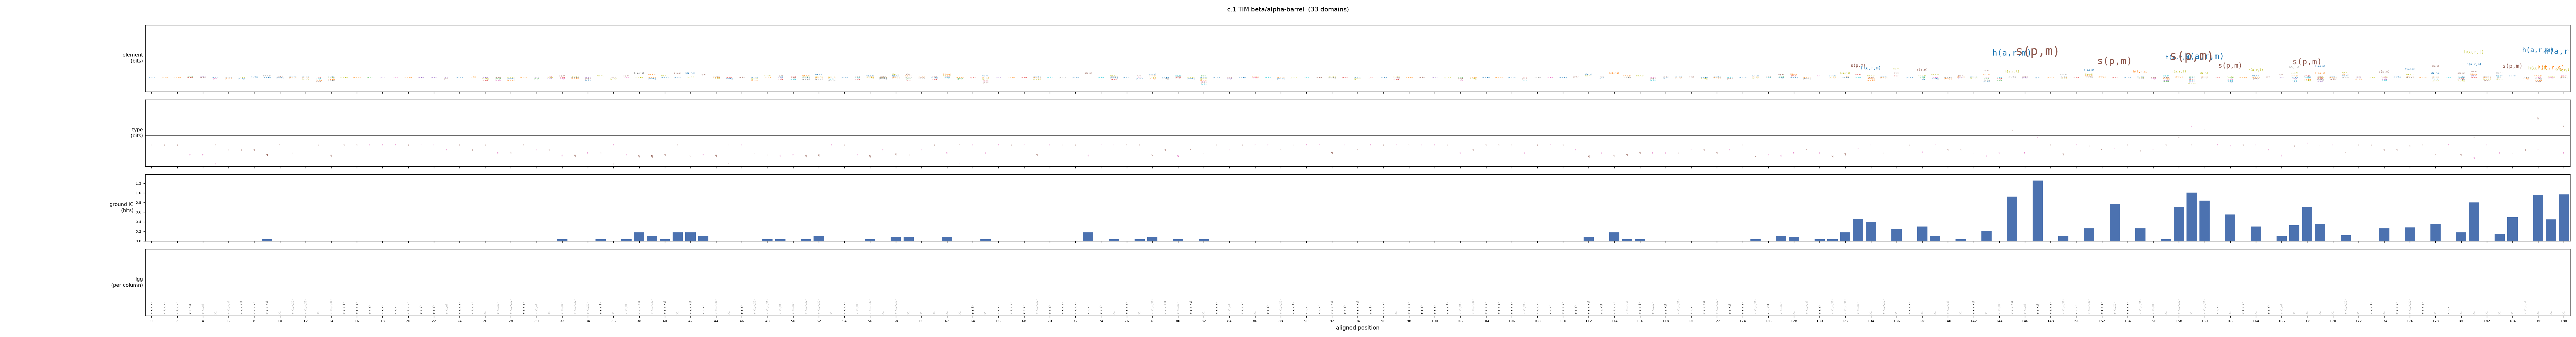
\includegraphics[width=0.96\textwidth]{figures/logo_tim_barrel.png}
  \end{center}
  \vspace{-0.4em}
  {\scriptsize SCOP fold \textbf{c.1 (TIM $\beta/\alpha$-barrel)} -- the conserved
  alternating parallel strands \atom{s(p,m)} and $\alpha$-helices, reconstructed
  by \code{examples/scop\_logos.py}.}
\end{frame}

\begin{frame}{Logos match the SCOP expert descriptions}
  \begin{center}
    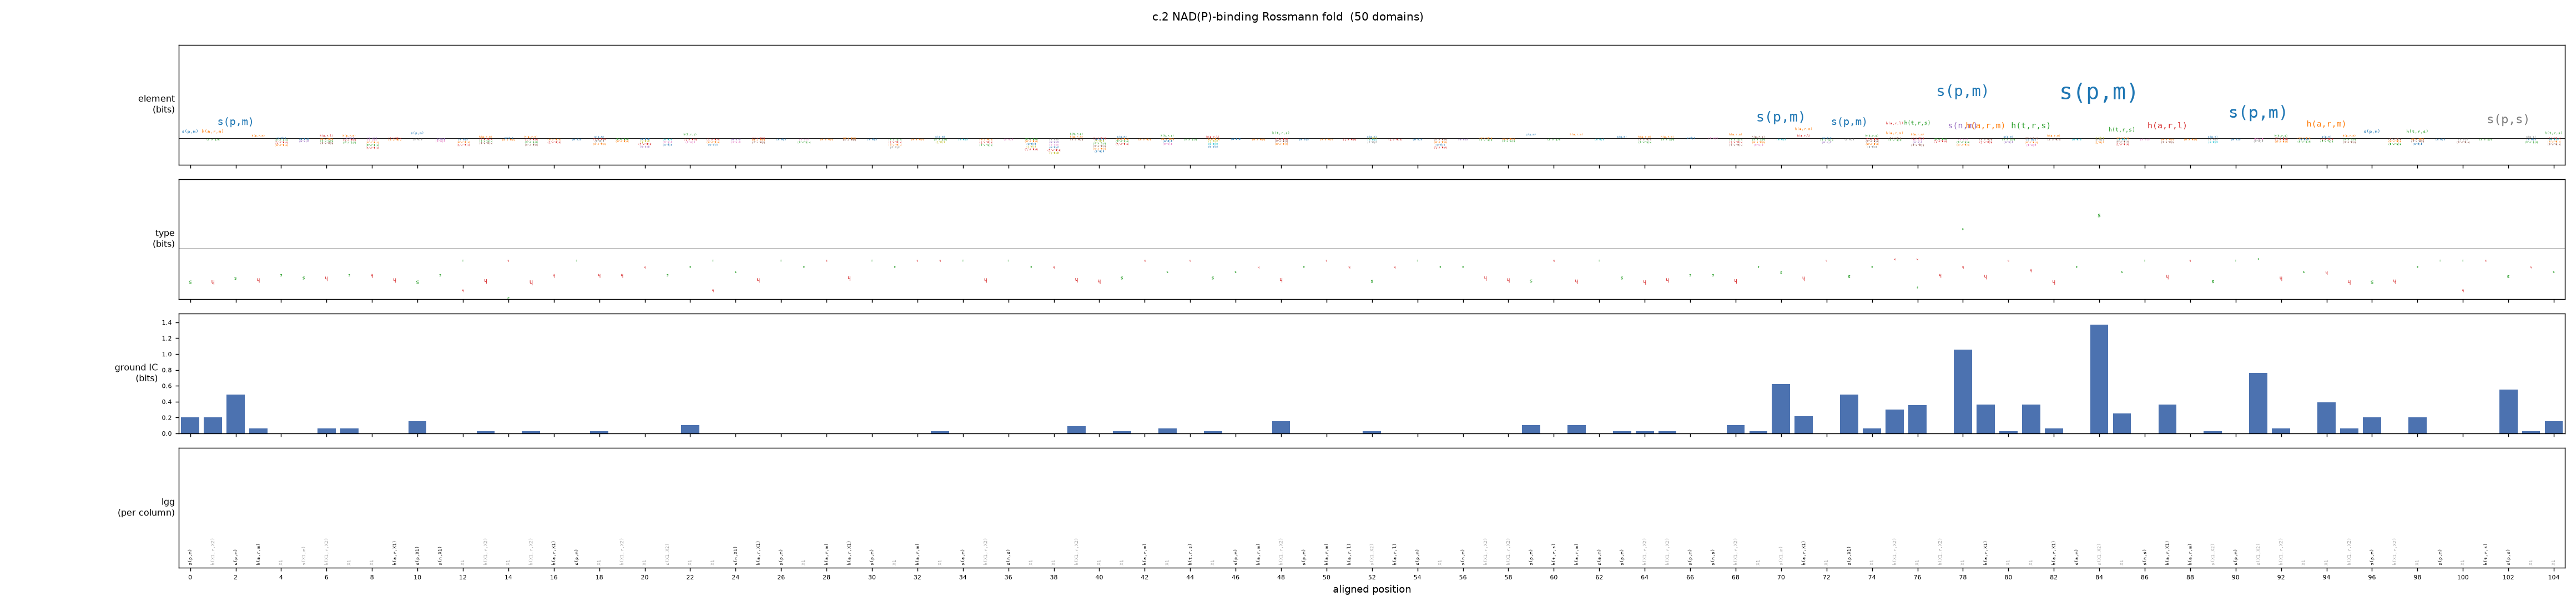
\includegraphics[width=0.97\textwidth]{figures/logo_rossmann.png}
  \end{center}
  \vspace{-0.3em}
  {\scriptsize SCOP fold \textbf{c.2 (NAD(P)-binding Rossmann fold)}: the
  information peaks fall on the conserved \alert{parallel $\beta$-strands}
  \atom{s(p,m)} -- exactly the ``6 parallel strands'' the SCOP database describes
  (paper Fig.~6). No learning involved -- pure alignment + IC.}
\end{frame}

\begin{frame}{The running example: balloon (NLP)}
  Five POS-tagged sentences (\atom{pred(word)} atoms) aligned and rendered as a
  logo: the shared syntactic skeleton \atom{dt nn nn vbd prp in in dt \dots}
  emerges at the abstract (part-of-speech) level.
  \begin{center}
    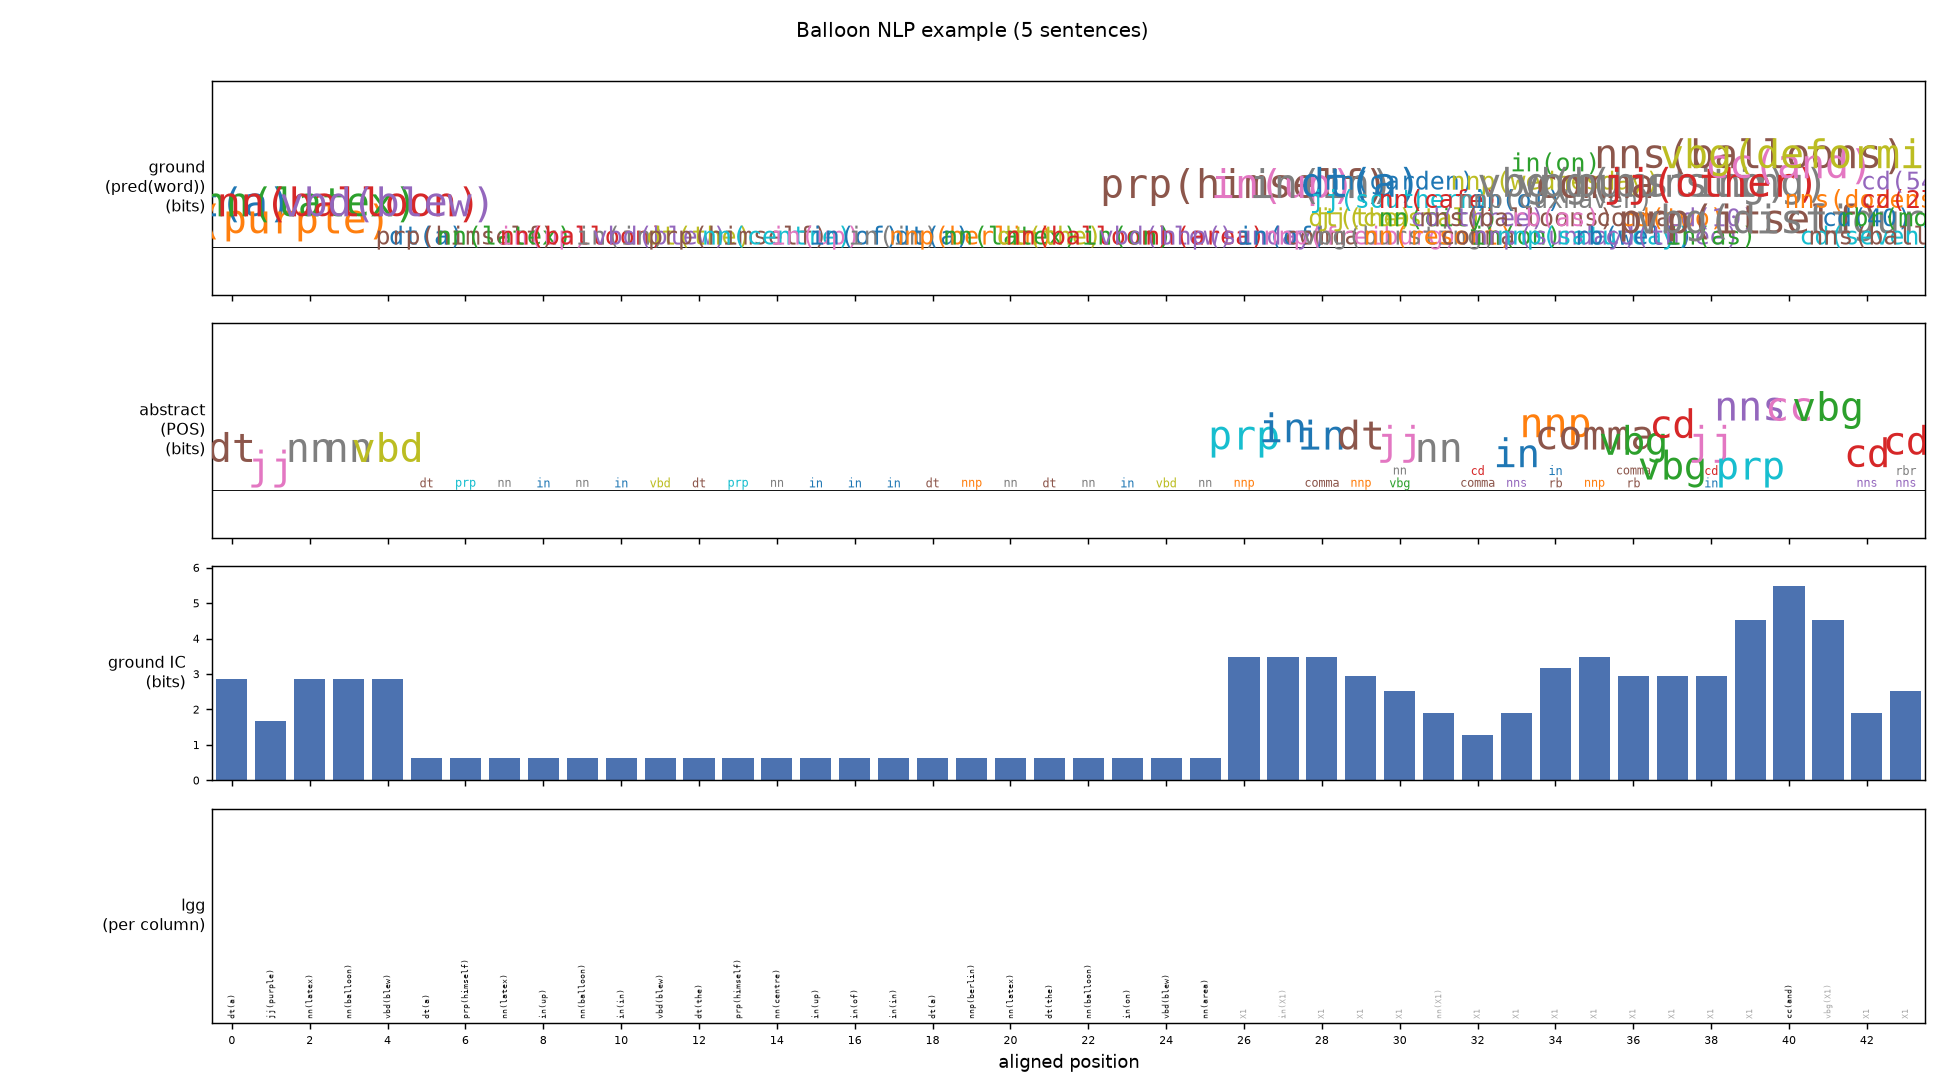
\includegraphics[width=0.99\textwidth]{figures/logo_balloon.png}
  \end{center}
  \vspace{-0.2em}
  \begin{columns}[c]
    \begin{column}{0.62\textwidth}
      {\scriptsize Total information content \textbf{81.8 bits}, matching the
      paper's reported \textbf{80.7} for the relational representation
      (Example~7) -- and above the flat 79.8.}
    \end{column}
    \begin{column}{0.36\textwidth}
      \centering\scriptsize
      \begin{tabular}{lc}
        \toprule
        representation & IC (bits)\\\midrule
        flat (paper) & 79.8\\
        relational (paper) & 80.7\\
        \textbf{pySeqAlign} & \textbf{81.8}\\
        \bottomrule
      \end{tabular}
    \end{column}
  \end{columns}
\end{frame}

% ============================================================
\section{Using it}
\begin{frame}[fragile]{Putting it together}
\small
\begin{verbatim}
from pyseqalign.msa import progressive_msa
from pyseqalign.logo import relational_logo
from pyseqalign.scoring.distance import AtomDistance

store = {1:('h','a','r','m'), 2:('s','p','m'), 3:('h','a','r','l')}
seqs  = {'d1':[1,2,3], 'd2':[1,3,2], 'd3':[2,3]}

sc  = AtomDistance(atom_store=store, gap_score=-0.5)  # NC distance
msa = progressive_msa(seqs, sc, gap_open=-1.0, gap_extend=-0.1)
relational_logo(list(msa.aligned_sequences.values()),
                store, 'logo.png', title='fold c.1')
\end{verbatim}
\normalsize
  \vspace{0.2em}
  {\scriptsize \code{pip install pyseqalignment} -- pure-Python core; the C++
  aligner is compiled automatically at install when a compiler is present, else
  it falls back silently.}
\end{frame}

% ============================================================
\begin{frame}{Summary}
  \begin{itemize}
    \item pySeqAlign aligns sequences of \textbf{structured logical atoms} with
          classic DP algorithms and an ILP relational distance.
    \item \textbf{MSA + relational logos} reproduce the ILP-2006 results
          standalone -- SCOP fold logos match the expert descriptions; the
          balloon logo reproduces the paper's information content.
    \item The scoring function is pluggable: the \alert{same} engine serves the
          fixed Nienhuys--Cheng distance and \textbf{pyREAL's learned rewards}.
    \item Pure-Python core; optional auto-compiled C++ accelerator.
  \end{itemize}
  \vspace{0.6em}
  \begin{center}
    \small \textbf{pyREAL} adds the learning $\rightarrow$ see the companion deck.
  \end{center}
\end{frame}

\end{document}
